\documentclass[1p]{elsarticle_modified}
%\bibliographystyle{elsarticle-num}

%\usepackage[colorlinks]{hyperref}
%\usepackage{abbrmath_seonhwa} %\Abb, \Ascr, \Acal ,\Abf, \Afrak
\usepackage{amsfonts}
\usepackage{amssymb}
\usepackage{amsmath}
\usepackage{amsthm}
\usepackage{scalefnt}
\usepackage{amsbsy}
\usepackage{kotex}
\usepackage{caption}
\usepackage{subfig}
\usepackage{color}
\usepackage{graphicx}
\usepackage{xcolor} %% white, black, red, green, blue, cyan, magenta, yellow
\usepackage{float}
\usepackage{setspace}
\usepackage{hyperref}

\usepackage{tikz}
\usetikzlibrary{arrows}

\usepackage{multirow}
\usepackage{array} % fixed length table
\usepackage{hhline}

%%%%%%%%%%%%%%%%%%%%%
\makeatletter
\renewcommand*\env@matrix[1][\arraystretch]{%
	\edef\arraystretch{#1}%
	\hskip -\arraycolsep
	\let\@ifnextchar\new@ifnextchar
	\array{*\c@MaxMatrixCols c}}
\makeatother %https://tex.stackexchange.com/questions/14071/how-can-i-increase-the-line-spacing-in-a-matrix
%%%%%%%%%%%%%%%

\usepackage[normalem]{ulem}

\newcommand{\msout}[1]{\ifmmode\text{\sout{\ensuremath{#1}}}\else\sout{#1}\fi}
%SOURCE: \msout is \stkout macro in https://tex.stackexchange.com/questions/20609/strikeout-in-math-mode

\newcommand{\cancel}[1]{
	\ifmmode
	{\color{red}\msout{#1}}
	\else
	{\color{red}\sout{#1}}
	\fi
}

\newcommand{\add}[1]{
	{\color{blue}\uwave{#1}}
}

\newcommand{\replace}[2]{
	\ifmmode
	{\color{red}\msout{#1}}{\color{blue}\uwave{#2}}
	\else
	{\color{red}\sout{#1}}{\color{blue}\uwave{#2}}
	\fi
}

\newcommand{\Sol}{\mathcal{S}} %segment
\newcommand{\D}{D} %diagram
\newcommand{\A}{\mathcal{A}} %arc


%%%%%%%%%%%%%%%%%%%%%%%%%%%%%5 test

\def\sl{\operatorname{\textup{SL}}(2,\Cbb)}
\def\psl{\operatorname{\textup{PSL}}(2,\Cbb)}
\def\quan{\mkern 1mu \triangleright \mkern 1mu}

\theoremstyle{definition}
\newtheorem{thm}{Theorem}[section]
\newtheorem{prop}[thm]{Proposition}
\newtheorem{lem}[thm]{Lemma}
\newtheorem{ques}[thm]{Question}
\newtheorem{cor}[thm]{Corollary}
\newtheorem{defn}[thm]{Definition}
\newtheorem{exam}[thm]{Example}
\newtheorem{rmk}[thm]{Remark}
\newtheorem{alg}[thm]{Algorithm}

\newcommand{\I}{\sqrt{-1}}
\begin{document}

%\begin{frontmatter}
%
%\title{Boundary parabolic representations of knots up to 8 crossings}
%
%%% Group authors per affiliation:
%\author{Yunhi Cho} 
%\address{Department of Mathematics, University of Seoul, Seoul, Korea}
%\ead{yhcho@uos.ac.kr}
%
%
%\author{Seonhwa Kim} %\fnref{s_kim}}
%\address{Center for Geometry and Physics, Institute for Basic Science, Pohang, 37673, Korea}
%\ead{ryeona17@ibs.re.kr}
%
%\author{Hyuk Kim}
%\address{Department of Mathematical Sciences, Seoul National University, Seoul 08826, Korea}
%\ead{hyukkim@snu.ac.kr}
%
%\author{Seokbeom Yoon}
%\address{Department of Mathematical Sciences, Seoul National University, Seoul, 08826,  Korea}
%\ead{sbyoon15@snu.ac.kr}
%
%\begin{abstract}
%We find all boundary parabolic representation of knots up to 8 crossings.
%
%\end{abstract}
%\begin{keyword}
%    \MSC[2010] 57M25 
%\end{keyword}
%
%\end{frontmatter}

%\linenumbers
%\tableofcontents
%
\newcommand\colored[1]{\textcolor{white}{\rule[-0.35ex]{0.8em}{1.4ex}}\kern-0.8em\color{red} #1}%
%\newcommand\colored[1]{\textcolor{white}{ #1}\kern-2.17ex	\textcolor{white}{ #1}\kern-1.81ex	\textcolor{white}{ #1}\kern-2.15ex\color{red}#1	}

{\Large $\underline{12n_{0330}~(K12n_{0330})}$}

\setlength{\tabcolsep}{10pt}
\renewcommand{\arraystretch}{1.6}
\vspace{1cm}\begin{tabular}{m{100pt}>{\centering\arraybackslash}m{274pt}}
\multirow{5}{120pt}{
	\centering
	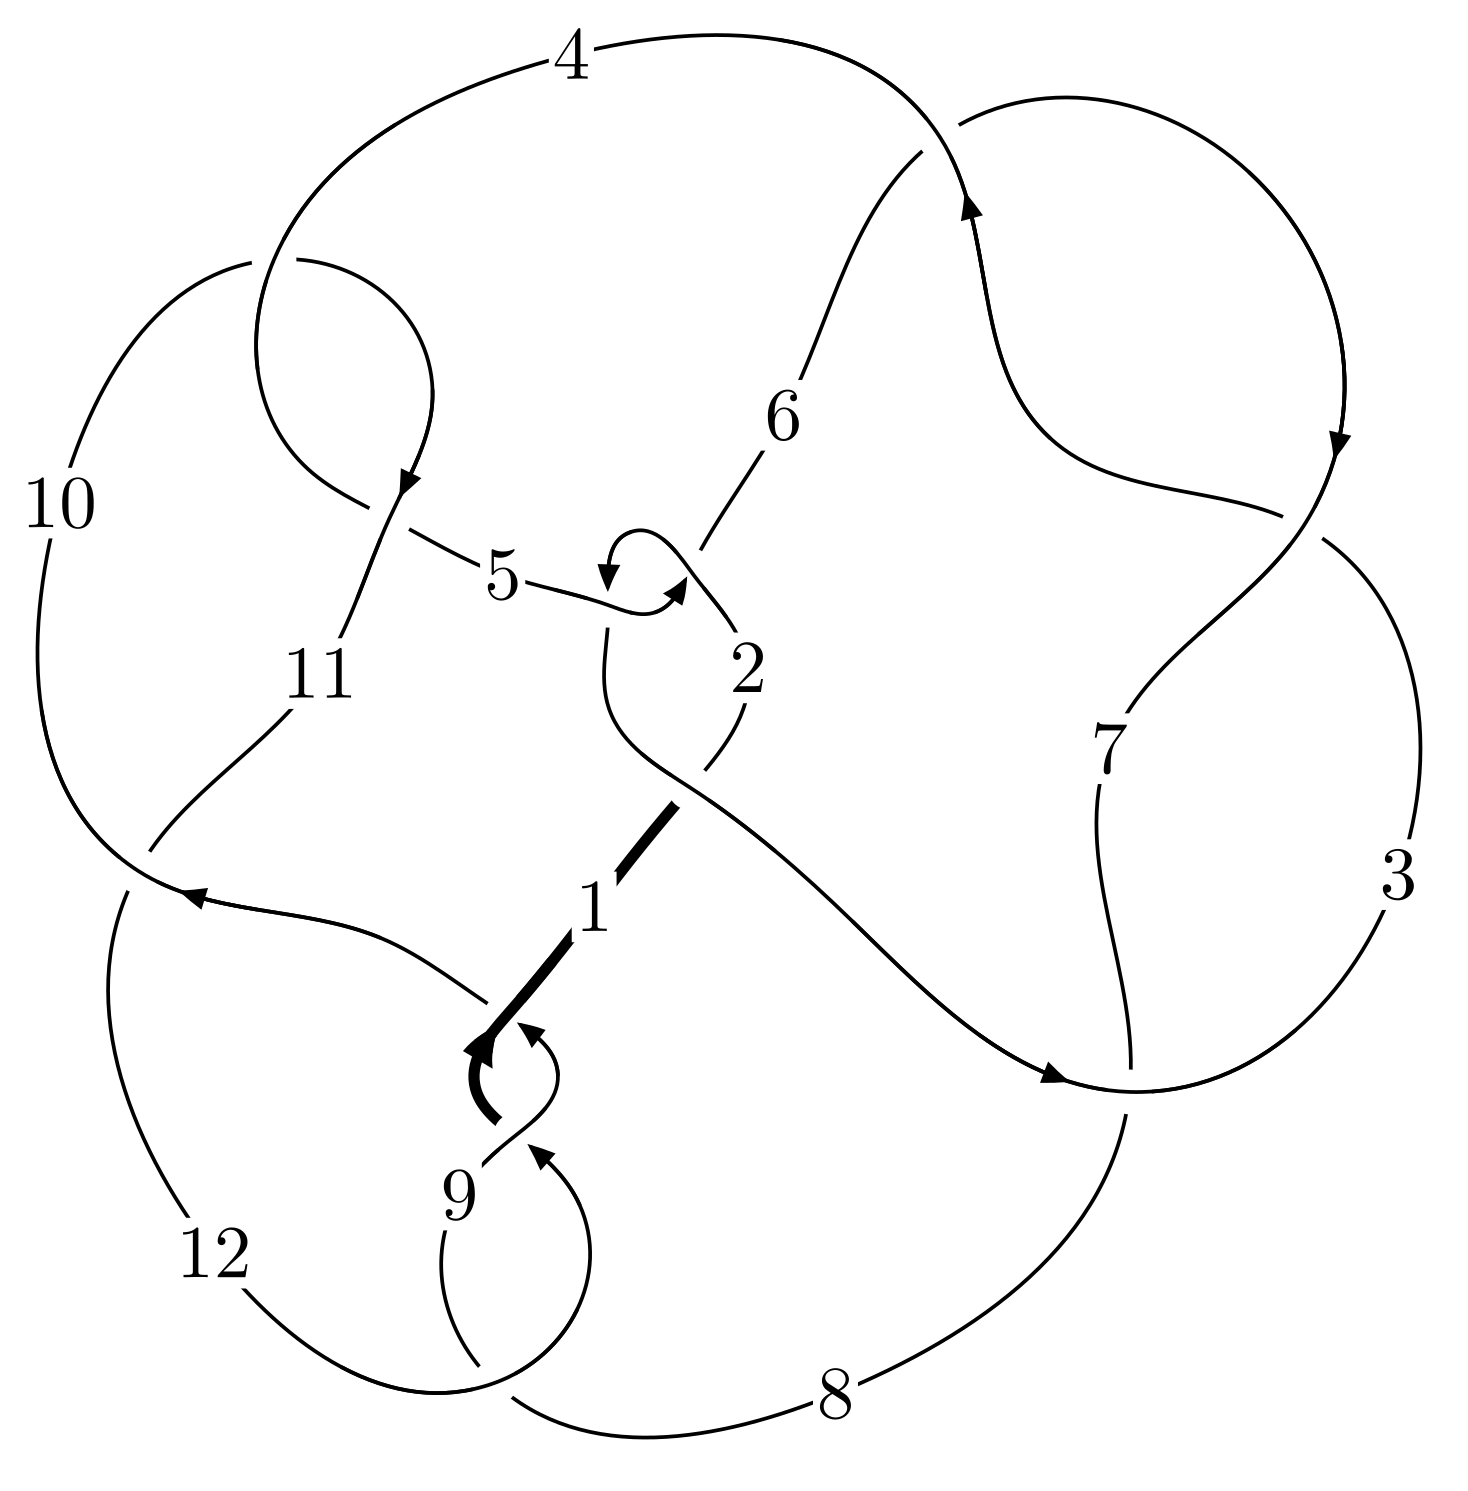
\includegraphics[width=112pt]{../../../GIT/diagram.site/Diagrams/png/2419_12n_0330.png}\\
\ \ \ A knot diagram\footnotemark}&
\allowdisplaybreaks
\textbf{Linearized knot diagam} \\
\cline{2-2}
 &
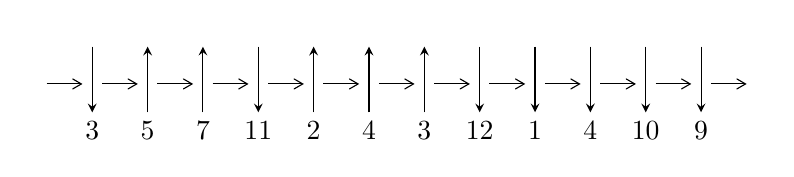
\begin{tikzpicture}[x=20pt, y=17pt]
	% nodes
	\node (C0) at (0, 0) {};
	\node (C1) at (1, 0) {};
	\node (C1U) at (1, +1) {};
	\node (C1D) at (1, -1) {3};

	\node (C2) at (2, 0) {};
	\node (C2U) at (2, +1) {};
	\node (C2D) at (2, -1) {5};

	\node (C3) at (3, 0) {};
	\node (C3U) at (3, +1) {};
	\node (C3D) at (3, -1) {7};

	\node (C4) at (4, 0) {};
	\node (C4U) at (4, +1) {};
	\node (C4D) at (4, -1) {11};

	\node (C5) at (5, 0) {};
	\node (C5U) at (5, +1) {};
	\node (C5D) at (5, -1) {2};

	\node (C6) at (6, 0) {};
	\node (C6U) at (6, +1) {};
	\node (C6D) at (6, -1) {4};

	\node (C7) at (7, 0) {};
	\node (C7U) at (7, +1) {};
	\node (C7D) at (7, -1) {3};

	\node (C8) at (8, 0) {};
	\node (C8U) at (8, +1) {};
	\node (C8D) at (8, -1) {12};

	\node (C9) at (9, 0) {};
	\node (C9U) at (9, +1) {};
	\node (C9D) at (9, -1) {1};

	\node (C10) at (10, 0) {};
	\node (C10U) at (10, +1) {};
	\node (C10D) at (10, -1) {4};

	\node (C11) at (11, 0) {};
	\node (C11U) at (11, +1) {};
	\node (C11D) at (11, -1) {10};

	\node (C12) at (12, 0) {};
	\node (C12U) at (12, +1) {};
	\node (C12D) at (12, -1) {9};
	\node (C13) at (13, 0) {};

	% arrows
	\draw[->,>={angle 60}]
	(C0) edge (C1) (C1) edge (C2) (C2) edge (C3) (C3) edge (C4) (C4) edge (C5) (C5) edge (C6) (C6) edge (C7) (C7) edge (C8) (C8) edge (C9) (C9) edge (C10) (C10) edge (C11) (C11) edge (C12) (C12) edge (C13) ;	\draw[->,>=stealth]
	(C1U) edge (C1D) (C2D) edge (C2U) (C3D) edge (C3U) (C4U) edge (C4D) (C5D) edge (C5U) (C6D) edge (C6U) (C7D) edge (C7U) (C8U) edge (C8D) (C9U) edge (C9D) (C10U) edge (C10D) (C11U) edge (C11D) (C12U) edge (C12D) ;
	\end{tikzpicture} \\
\hhline{~~} \\& 
\textbf{Solving Sequence} \\ \cline{2-2} 
 &
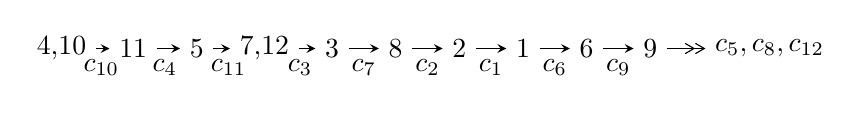
\begin{tikzpicture}[x=23pt, y=7pt]
	% node
	\node (A0) at (-1/8, 0) {4,10};
	\node (A1) at (1, 0) {11};
	\node (A2) at (2, 0) {5};
	\node (A3) at (49/16, 0) {7,12};
	\node (A4) at (33/8, 0) {3};
	\node (A5) at (41/8, 0) {8};
	\node (A6) at (49/8, 0) {2};
	\node (A7) at (57/8, 0) {1};
	\node (A8) at (65/8, 0) {6};
	\node (A9) at (73/8, 0) {9};
	\node (C1) at (1/2, -1) {$c_{10}$};
	\node (C2) at (3/2, -1) {$c_{4}$};
	\node (C3) at (5/2, -1) {$c_{11}$};
	\node (C4) at (29/8, -1) {$c_{3}$};
	\node (C5) at (37/8, -1) {$c_{7}$};
	\node (C6) at (45/8, -1) {$c_{2}$};
	\node (C7) at (53/8, -1) {$c_{1}$};
	\node (C8) at (61/8, -1) {$c_{6}$};
	\node (C9) at (69/8, -1) {$c_{9}$};
	\node (A10) at (11, 0) {$c_{5},c_{8},c_{12}$};

	% edge
	\draw[->,>=stealth]	
	(A0) edge (A1) (A1) edge (A2) (A2) edge (A3) (A3) edge (A4) (A4) edge (A5) (A5) edge (A6) (A6) edge (A7) (A7) edge (A8) (A8) edge (A9) ;
	\draw[->>,>={angle 60}]	
	(A9) edge (A10);
\end{tikzpicture} \\ 

\end{tabular} \\

\footnotetext{
The image of knot diagram is generated by the software ``\textbf{Draw programme}" developed by Andrew Bartholomew(\url{http://www.layer8.co.uk/maths/draw/index.htm\#Running-draw}), where we modified some parts for our purpose(\url{https://github.com/CATsTAILs/LinksPainter}).
}\phantom \\ \newline 
\centering \textbf{Ideals for irreducible components\footnotemark of $X_{\text{par}}$} 
 
\begin{align*}
I^u_{1}&=\langle 
7.74526\times10^{16} u^{25}-1.33763\times10^{17} u^{24}+\cdots+7.07898\times10^{18} b+5.73871\times10^{18},\\
\phantom{I^u_{1}}&\phantom{= \langle  }-6.55698\times10^{18} u^{25}+2.22473\times10^{19} u^{24}+\cdots+1.41580\times10^{19} a-1.02368\times10^{20},\;u^{26}-3 u^{25}+\cdots+6 u+8\rangle \\
I^u_{2}&=\langle 
u^{13}+u^{12}- u^{11}-2 u^{10}+4 u^9+5 u^8-3 u^7-6 u^6+4 u^5+6 u^4- u^2 a-2 u^3-2 u^2+b+a+2 u+1,\\
\phantom{I^u_{2}}&\phantom{= \langle  }u^{13}+2 u^{12}-3 u^{10}+2 u^9+9 u^8+2 u^7-9 u^6-2 u^5+10 u^4+4 u^3+a^2+a u-3 u^2+3,\\
\phantom{I^u_{2}}&\phantom{= \langle  }u^{14}+u^{13}- u^{12}-2 u^{11}+4 u^{10}+5 u^9-3 u^8-6 u^7+4 u^6+6 u^5-2 u^4-2 u^3+2 u^2+u-1\rangle \\
I^u_{3}&=\langle 
- u^9+u^8+3 u^7-2 u^6-4 u^5+u^4+u^3+2 u^2+b+u-1,\;- u^8+2 u^6- u^4-2 u^2+a+1,\\
\phantom{I^u_{3}}&\phantom{= \langle  }u^{10}-3 u^8+4 u^6- u^4- u^2+1\rangle \\
\\
I^v_{1}&=\langle 
a,\;2 b+1,\;v-2\rangle \\
\end{align*}
\raggedright * 4 irreducible components of $\dim_{\mathbb{C}}=0$, with total 65 representations.\\
\footnotetext{All coefficients of polynomials are rational numbers. But the coefficients are sometimes approximated in decimal forms when there is not enough margin.}
\newpage
\renewcommand{\arraystretch}{1}
\centering \section*{I. $I^u_{1}= \langle 7.75\times10^{16} u^{25}-1.34\times10^{17} u^{24}+\cdots+7.08\times10^{18} b+5.74\times10^{18},\;-6.56\times10^{18} u^{25}+2.22\times10^{19} u^{24}+\cdots+1.42\times10^{19} a-1.02\times10^{20},\;u^{26}-3 u^{25}+\cdots+6 u+8 \rangle$}
\flushleft \textbf{(i) Arc colorings}\\
\begin{tabular}{m{7pt} m{180pt} m{7pt} m{180pt} }
\flushright $a_{4}=$&$\begin{pmatrix}0\\u\end{pmatrix}$ \\
\flushright $a_{10}=$&$\begin{pmatrix}1\\0\end{pmatrix}$ \\
\flushright $a_{11}=$&$\begin{pmatrix}1\\u^2\end{pmatrix}$ \\
\flushright $a_{5}=$&$\begin{pmatrix}- u\\- u^3+u\end{pmatrix}$ \\
\flushright $a_{7}=$&$\begin{pmatrix}0.463130 u^{25}-1.57137 u^{24}+\cdots-7.38977 u+7.23041\\-0.0109412 u^{25}+0.0188959 u^{24}+\cdots+0.948527 u-0.810670\end{pmatrix}$ \\
\flushright $a_{12}=$&$\begin{pmatrix}- u^2+1\\u^2\end{pmatrix}$ \\
\flushright $a_{3}=$&$\begin{pmatrix}-0.452189 u^{25}+1.55247 u^{24}+\cdots+6.44124 u-6.41974\\-0.139816 u^{25}+0.520475 u^{24}+\cdots+3.39062 u-2.37790\end{pmatrix}$ \\
\flushright $a_{8}=$&$\begin{pmatrix}1.05514 u^{25}-3.64431 u^{24}+\cdots-16.2216 u+16.0280\\0.00913190 u^{25}-0.0544808 u^{24}+\cdots+0.384691 u-0.813121\end{pmatrix}$ \\
\flushright $a_{2}=$&$\begin{pmatrix}-0.257452 u^{25}+0.942913 u^{24}+\cdots+3.82805 u-4.96393\\-0.288157 u^{25}+0.949849 u^{24}+\cdots+4.59799 u-3.63094\end{pmatrix}$ \\
\flushright $a_{1}=$&$\begin{pmatrix}-1.06427 u^{25}+3.69879 u^{24}+\cdots+15.8369 u-15.2149\\-0.283474 u^{25}+1.06311 u^{24}+\cdots+5.86288 u-4.86106\end{pmatrix}$ \\
\flushright $a_{6}=$&$\begin{pmatrix}0.463130 u^{25}-1.57137 u^{24}+\cdots-7.38977 u+7.23041\\0.183796 u^{25}-0.590662 u^{24}+\cdots-1.66466 u+0.645138\end{pmatrix}$ \\
\flushright $a_{9}=$&$\begin{pmatrix}1.28428 u^{25}-4.51273 u^{24}+\cdots-21.0928 u+19.1876\\0.0634646 u^{25}-0.249171 u^{24}+\cdots-0.606969 u+0.888390\end{pmatrix}$\\&\end{tabular}
\flushleft \textbf{(ii) Obstruction class $= -1$}\\~\\
\flushleft \textbf{(iii) Cusp Shapes $= \frac{2235431246280387471}{2022564411084206648} u^{25}-\frac{50383957546292106623}{14157950877589446536} u^{24}+\cdots-\frac{96855145260069592069}{14157950877589446536} u+\frac{73272041333640892293}{7078975438794723268}$}\\~\\
\newpage\renewcommand{\arraystretch}{1}
\flushleft \textbf{(iv) u-Polynomials at the component}\newline \\
\begin{tabular}{m{50pt}|m{274pt}}
Crossings & \hspace{64pt}u-Polynomials at each crossing \\
\hline $$\begin{aligned}c_{1}\end{aligned}$$&$\begin{aligned}
&u^{26}+5 u^{25}+\cdots-5 u+1
\end{aligned}$\\
\hline $$\begin{aligned}c_{2},c_{3},c_{5}\\c_{6},c_{7}\end{aligned}$$&$\begin{aligned}
&u^{26}- u^{25}+\cdots-3 u-1
\end{aligned}$\\
\hline $$\begin{aligned}c_{4},c_{10}\end{aligned}$$&$\begin{aligned}
&u^{26}-3 u^{25}+\cdots+6 u+8
\end{aligned}$\\
\hline $$\begin{aligned}c_{8},c_{9},c_{12}\end{aligned}$$&$\begin{aligned}
&u^{26}-2 u^{25}+\cdots+7 u-4
\end{aligned}$\\
\hline $$\begin{aligned}c_{11}\end{aligned}$$&$\begin{aligned}
&u^{26}+9 u^{25}+\cdots+436 u+64
\end{aligned}$\\
\hline
\end{tabular}\\~\\
\newpage\renewcommand{\arraystretch}{1}
\flushleft \textbf{(v) Riley Polynomials at the component}\newline \\
\begin{tabular}{m{50pt}|m{274pt}}
Crossings & \hspace{64pt}Riley Polynomials at each crossing \\
\hline $$\begin{aligned}c_{1}\end{aligned}$$&$\begin{aligned}
&y^{26}+37 y^{25}+\cdots-157 y+1
\end{aligned}$\\
\hline $$\begin{aligned}c_{2},c_{3},c_{5}\\c_{6},c_{7}\end{aligned}$$&$\begin{aligned}
&y^{26}+5 y^{25}+\cdots-5 y+1
\end{aligned}$\\
\hline $$\begin{aligned}c_{4},c_{10}\end{aligned}$$&$\begin{aligned}
&y^{26}-9 y^{25}+\cdots-436 y+64
\end{aligned}$\\
\hline $$\begin{aligned}c_{8},c_{9},c_{12}\end{aligned}$$&$\begin{aligned}
&y^{26}-22 y^{25}+\cdots-65 y+16
\end{aligned}$\\
\hline $$\begin{aligned}c_{11}\end{aligned}$$&$\begin{aligned}
&y^{26}+15 y^{25}+\cdots-142352 y+4096
\end{aligned}$\\
\hline
\end{tabular}\\~\\
\newpage\flushleft \textbf{(vi) Complex Volumes and Cusp Shapes}
$$\begin{array}{c|c|c}  
\text{Solutions to }I^u_{1}& \I (\text{vol} + \sqrt{-1}CS) & \text{Cusp shape}\\
 \hline 
\begin{aligned}
u &= -0.982745 + 0.211485 I \\
a &= \phantom{-}0.402843 - 0.499085 I \\
b &= -0.232498 + 0.875894 I\end{aligned}
 & -1.77257 + 0.70535 I & -4.40558 + 0.51415 I \\ \hline\begin{aligned}
u &= -0.982745 - 0.211485 I \\
a &= \phantom{-}0.402843 + 0.499085 I \\
b &= -0.232498 - 0.875894 I\end{aligned}
 & -1.77257 - 0.70535 I & -4.40558 - 0.51415 I \\ \hline\begin{aligned}
u &= \phantom{-}0.010508 + 1.069030 I \\
a &= -0.600779 - 0.379610 I \\
b &= \phantom{-}0.115449 + 0.616202 I\end{aligned}
 & -3.79097 - 1.46714 I & -5.06055 + 4.75413 I \\ \hline\begin{aligned}
u &= \phantom{-}0.010508 - 1.069030 I \\
a &= -0.600779 + 0.379610 I \\
b &= \phantom{-}0.115449 - 0.616202 I\end{aligned}
 & -3.79097 + 1.46714 I & -5.06055 - 4.75413 I \\ \hline\begin{aligned}
u &= \phantom{-}0.734341 + 0.797765 I \\
a &= \phantom{-}1.257320 - 0.172643 I \\
b &= \phantom{-}0.228017 + 1.091210 I\end{aligned}
 & \phantom{-}2.81865 - 0.76966 I & -3.02229 + 2.23661 I \\ \hline\begin{aligned}
u &= \phantom{-}0.734341 - 0.797765 I \\
a &= \phantom{-}1.257320 + 0.172643 I \\
b &= \phantom{-}0.228017 - 1.091210 I\end{aligned}
 & \phantom{-}2.81865 + 0.76966 I & -3.02229 - 2.23661 I \\ \hline\begin{aligned}
u &= \phantom{-}1.074650 + 0.168126 I \\
a &= -0.355808 + 0.706778 I \\
b &= \phantom{-}0.039591 - 1.309980 I\end{aligned}
 & -1.79599 - 3.76105 I & -4.80263 + 8.00937 I \\ \hline\begin{aligned}
u &= \phantom{-}1.074650 - 0.168126 I \\
a &= -0.355808 - 0.706778 I \\
b &= \phantom{-}0.039591 + 1.309980 I\end{aligned}
 & -1.79599 + 3.76105 I & -4.80263 - 8.00937 I \\ \hline\begin{aligned}
u &= -0.745967 + 0.945276 I \\
a &= -1.129930 - 0.091852 I \\
b &= -0.012396 + 1.135900 I\end{aligned}
 & \phantom{-}6.07946 - 3.67877 I & -0.12041 + 2.47120 I \\ \hline\begin{aligned}
u &= -0.745967 - 0.945276 I \\
a &= -1.129930 + 0.091852 I \\
b &= -0.012396 - 1.135900 I\end{aligned}
 & \phantom{-}6.07946 + 3.67877 I & -0.12041 - 2.47120 I\\
 \hline 
 \end{array}$$\newpage$$\begin{array}{c|c|c}  
\text{Solutions to }I^u_{1}& \I (\text{vol} + \sqrt{-1}CS) & \text{Cusp shape}\\
 \hline 
\begin{aligned}
u &= \phantom{-}1.021750 + 0.716695 I \\
a &= -0.081674 + 1.052890 I \\
b &= -0.92093 - 2.01835 I\end{aligned}
 & \phantom{-}1.91220 - 4.97774 I & -4.59322 + 4.08967 I \\ \hline\begin{aligned}
u &= \phantom{-}1.021750 - 0.716695 I \\
a &= -0.081674 - 1.052890 I \\
b &= -0.92093 + 2.01835 I\end{aligned}
 & \phantom{-}1.91220 + 4.97774 I & -4.59322 - 4.08967 I \\ \hline\begin{aligned}
u &= \phantom{-}0.755105 + 1.061790 I \\
a &= \phantom{-}1.036650 - 0.033748 I \\
b &= -0.151747 + 1.120760 I\end{aligned}
 & \phantom{-}1.48699 + 8.04356 I & -4.72322 - 5.24092 I \\ \hline\begin{aligned}
u &= \phantom{-}0.755105 - 1.061790 I \\
a &= \phantom{-}1.036650 + 0.033748 I \\
b &= -0.151747 - 1.120760 I\end{aligned}
 & \phantom{-}1.48699 - 8.04356 I & -4.72322 + 5.24092 I \\ \hline\begin{aligned}
u &= -1.062230 + 0.805325 I \\
a &= -0.007950 + 1.055910 I \\
b &= \phantom{-}1.20574 - 1.93593 I\end{aligned}
 & \phantom{-}5.07466 + 10.13450 I & -2.10298 - 6.96057 I \\ \hline\begin{aligned}
u &= -1.062230 - 0.805325 I \\
a &= -0.007950 - 1.055910 I \\
b &= \phantom{-}1.20574 + 1.93593 I\end{aligned}
 & \phantom{-}5.07466 - 10.13450 I & -2.10298 + 6.96057 I \\ \hline\begin{aligned}
u &= \phantom{-}1.279790 + 0.462764 I \\
a &= -0.302749 - 0.444518 I \\
b &= \phantom{-}0.042614 + 0.739956 I\end{aligned}
 & -7.94739 - 3.73170 I & -5.56768 - 0.86519 I \\ \hline\begin{aligned}
u &= \phantom{-}1.279790 - 0.462764 I \\
a &= -0.302749 + 0.444518 I \\
b &= \phantom{-}0.042614 - 0.739956 I\end{aligned}
 & -7.94739 + 3.73170 I & -5.56768 + 0.86519 I \\ \hline\begin{aligned}
u &= \phantom{-}0.175064 + 0.597925 I \\
a &= \phantom{-}0.812678 - 0.972268 I \\
b &= \phantom{-}0.082343 + 0.525293 I\end{aligned}
 & \phantom{-}1.28130 + 0.88301 I & \phantom{-}4.68220 - 2.63665 I \\ \hline\begin{aligned}
u &= \phantom{-}0.175064 - 0.597925 I \\
a &= \phantom{-}0.812678 + 0.972268 I \\
b &= \phantom{-}0.082343 - 0.525293 I\end{aligned}
 & \phantom{-}1.28130 - 0.88301 I & \phantom{-}4.68220 + 2.63665 I\\
 \hline 
 \end{array}$$\newpage$$\begin{array}{c|c|c}  
\text{Solutions to }I^u_{1}& \I (\text{vol} + \sqrt{-1}CS) & \text{Cusp shape}\\
 \hline 
\begin{aligned}
u &= -1.355470 + 0.349551 I \\
a &= \phantom{-}0.160592 + 0.704597 I \\
b &= \phantom{-}0.398277 - 1.175870 I\end{aligned}
 & -8.58893 + 6.63218 I & -8.67236 - 8.09999 I \\ \hline\begin{aligned}
u &= -1.355470 - 0.349551 I \\
a &= \phantom{-}0.160592 - 0.704597 I \\
b &= \phantom{-}0.398277 + 1.175870 I\end{aligned}
 & -8.58893 - 6.63218 I & -8.67236 + 8.09999 I \\ \hline\begin{aligned}
u &= \phantom{-}1.109820 + 0.856025 I \\
a &= \phantom{-}0.068276 + 1.033520 I \\
b &= -1.36937 - 1.78727 I\end{aligned}
 & \phantom{-}0.3265 - 14.9979 I & -5.89395 + 8.70861 I \\ \hline\begin{aligned}
u &= \phantom{-}1.109820 - 0.856025 I \\
a &= \phantom{-}0.068276 - 1.033520 I \\
b &= -1.36937 + 1.78727 I\end{aligned}
 & \phantom{-}0.3265 + 14.9979 I & -5.89395 - 8.70861 I \\ \hline\begin{aligned}
u &= -0.541106\phantom{ +0.000000I} \\
a &= -2.33904\phantom{ +0.000000I} \\
b &= -0.621412\phantom{ +0.000000I}\end{aligned}
 & -0.468550\phantom{ +0.000000I} & -16.1730\phantom{ +0.000000I} \\ \hline\begin{aligned}
u &= -0.488142\phantom{ +0.000000I} \\
a &= \phantom{-}0.570097\phantom{ +0.000000I} \\
b &= -0.728748\phantom{ +0.000000I}\end{aligned}
 & -1.21370\phantom{ +0.000000I} & -9.51190\phantom{ +0.000000I}\\
 \hline 
 \end{array}$$\newpage\newpage\renewcommand{\arraystretch}{1}
\centering \section*{II. $I^u_{2}= \langle u^{13}+u^{12}+\cdots+a+1,\;u^{13}+2 u^{12}+\cdots+a^2+3,\;u^{14}+u^{13}+\cdots+u-1 \rangle$}
\flushleft \textbf{(i) Arc colorings}\\
\begin{tabular}{m{7pt} m{180pt} m{7pt} m{180pt} }
\flushright $a_{4}=$&$\begin{pmatrix}0\\u\end{pmatrix}$ \\
\flushright $a_{10}=$&$\begin{pmatrix}1\\0\end{pmatrix}$ \\
\flushright $a_{11}=$&$\begin{pmatrix}1\\u^2\end{pmatrix}$ \\
\flushright $a_{5}=$&$\begin{pmatrix}- u\\- u^3+u\end{pmatrix}$ \\
\flushright $a_{7}=$&$\begin{pmatrix}a\\- u^{13}- u^{12}+\cdots- a-1\end{pmatrix}$ \\
\flushright $a_{12}=$&$\begin{pmatrix}- u^2+1\\u^2\end{pmatrix}$ \\
\flushright $a_{3}=$&$\begin{pmatrix}u^{13}+u^{12}+\cdots+2 u+1\\- u^{13}- u^{12}+\cdots+a-1\end{pmatrix}$ \\
\flushright $a_{8}=$&$\begin{pmatrix}u^5+u\\u^7- u^5+2 u^3- u\end{pmatrix}$ \\
\flushright $a_{2}=$&$\begin{pmatrix}u^{13}+u^{12}+\cdots+2 u+1\\- u^{13}- u^{12}+\cdots+a-1\end{pmatrix}$ \\
\flushright $a_{1}=$&$\begin{pmatrix}- u^7-2 u^3\\- u^9+u^7-3 u^5+2 u^3- u\end{pmatrix}$ \\
\flushright $a_{6}=$&$\begin{pmatrix}a\\- u^{13}- u^{12}+\cdots- a-1\end{pmatrix}$ \\
\flushright $a_{9}=$&$\begin{pmatrix}- u^{11}+2 u^9-4 u^7+6 u^5-3 u^3+2 u\\u^{11}- u^9+4 u^7-3 u^5+3 u^3- u\end{pmatrix}$\\&\end{tabular}
\flushleft \textbf{(ii) Obstruction class $= -1$}\\~\\
\flushleft \textbf{(iii) Cusp Shapes $= -4 u^{12}-4 u^{11}+4 u^{10}+8 u^9-16 u^8-16 u^7+12 u^6+20 u^5-16 u^4-12 u^3+8 u^2-10$}\\~\\
\newpage\renewcommand{\arraystretch}{1}
\flushleft \textbf{(iv) u-Polynomials at the component}\newline \\
\begin{tabular}{m{50pt}|m{274pt}}
Crossings & \hspace{64pt}u-Polynomials at each crossing \\
\hline $$\begin{aligned}c_{1}\end{aligned}$$&$\begin{aligned}
&u^{28}+11 u^{27}+\cdots+2888 u+289
\end{aligned}$\\
\hline $$\begin{aligned}c_{2},c_{3},c_{5}\\c_{6},c_{7}\end{aligned}$$&$\begin{aligned}
&u^{28}+3 u^{27}+\cdots+74 u+17
\end{aligned}$\\
\hline $$\begin{aligned}c_{4},c_{10}\end{aligned}$$&$\begin{aligned}
&(u^{14}+u^{13}+\cdots+u-1)^{2}
\end{aligned}$\\
\hline $$\begin{aligned}c_{8},c_{9},c_{12}\end{aligned}$$&$\begin{aligned}
&(u^{14}- u^{13}+\cdots-3 u-1)^{2}
\end{aligned}$\\
\hline $$\begin{aligned}c_{11}\end{aligned}$$&$\begin{aligned}
&(u^{14}+3 u^{13}+\cdots+5 u+1)^{2}
\end{aligned}$\\
\hline
\end{tabular}\\~\\
\newpage\renewcommand{\arraystretch}{1}
\flushleft \textbf{(v) Riley Polynomials at the component}\newline \\
\begin{tabular}{m{50pt}|m{274pt}}
Crossings & \hspace{64pt}Riley Polynomials at each crossing \\
\hline $$\begin{aligned}c_{1}\end{aligned}$$&$\begin{aligned}
&y^{28}+11 y^{27}+\cdots+1428812 y+83521
\end{aligned}$\\
\hline $$\begin{aligned}c_{2},c_{3},c_{5}\\c_{6},c_{7}\end{aligned}$$&$\begin{aligned}
&y^{28}+11 y^{27}+\cdots+2888 y+289
\end{aligned}$\\
\hline $$\begin{aligned}c_{4},c_{10}\end{aligned}$$&$\begin{aligned}
&(y^{14}-3 y^{13}+\cdots-5 y+1)^{2}
\end{aligned}$\\
\hline $$\begin{aligned}c_{8},c_{9},c_{12}\end{aligned}$$&$\begin{aligned}
&(y^{14}-11 y^{13}+\cdots-5 y+1)^{2}
\end{aligned}$\\
\hline $$\begin{aligned}c_{11}\end{aligned}$$&$\begin{aligned}
&(y^{14}+17 y^{13}+\cdots- y+1)^{2}
\end{aligned}$\\
\hline
\end{tabular}\\~\\
\newpage\flushleft \textbf{(vi) Complex Volumes and Cusp Shapes}
$$\begin{array}{c|c|c}  
\text{Solutions to }I^u_{2}& \I (\text{vol} + \sqrt{-1}CS) & \text{Cusp shape}\\
 \hline 
\begin{aligned}
u &= \phantom{-}0.919323 + 0.470231 I \\
a &= -0.404207 + 0.774825 I \\
b &= -1.380120 - 0.199773 I\end{aligned}
 & -6.26948 - 4.88256 I & -7.68599 + 6.44337 I \\ \hline\begin{aligned}
u &= \phantom{-}0.919323 + 0.470231 I \\
a &= -0.515117 - 1.245060 I \\
b &= \phantom{-}0.407942 + 0.463734 I\end{aligned}
 & -6.26948 - 4.88256 I & -7.68599 + 6.44337 I \\ \hline\begin{aligned}
u &= \phantom{-}0.919323 - 0.470231 I \\
a &= -0.404207 - 0.774825 I \\
b &= -1.380120 + 0.199773 I\end{aligned}
 & -6.26948 + 4.88256 I & -7.68599 - 6.44337 I \\ \hline\begin{aligned}
u &= \phantom{-}0.919323 - 0.470231 I \\
a &= -0.515117 + 1.245060 I \\
b &= \phantom{-}0.407942 - 0.463734 I\end{aligned}
 & -6.26948 + 4.88256 I & -7.68599 - 6.44337 I \\ \hline\begin{aligned}
u &= -0.924961\phantom{ +0.000000I} \\
a &= \phantom{-}0.46248 + 1.34555 I \\
b &= \phantom{-}1.014320 - 0.194361 I\end{aligned}
 & -8.84982\phantom{ +0.000000I} & -12.7050\phantom{ +0.000000I} \\ \hline\begin{aligned}
u &= -0.924961\phantom{ +0.000000I} \\
a &= \phantom{-}0.46248 - 1.34555 I \\
b &= \phantom{-}1.014320 + 0.194361 I\end{aligned}
 & -8.84982\phantom{ +0.000000I} & -12.7050\phantom{ +0.000000I} \\ \hline\begin{aligned}
u &= -0.726911 + 0.518054 I \\
a &= \phantom{-}0.725706 - 1.116820 I \\
b &= -0.465841 + 0.930039 I\end{aligned}
 & -1.93761 + 1.98638 I & -0.65592 - 5.08636 I \\ \hline\begin{aligned}
u &= -0.726911 + 0.518054 I \\
a &= \phantom{-}0.001206 + 0.598768 I \\
b &= \phantom{-}1.362390 + 0.206201 I\end{aligned}
 & -1.93761 + 1.98638 I & -0.65592 - 5.08636 I \\ \hline\begin{aligned}
u &= -0.726911 - 0.518054 I \\
a &= \phantom{-}0.725706 + 1.116820 I \\
b &= -0.465841 - 0.930039 I\end{aligned}
 & -1.93761 - 1.98638 I & -0.65592 + 5.08636 I \\ \hline\begin{aligned}
u &= -0.726911 - 0.518054 I \\
a &= \phantom{-}0.001206 - 0.598768 I \\
b &= \phantom{-}1.362390 - 0.206201 I\end{aligned}
 & -1.93761 - 1.98638 I & -0.65592 + 5.08636 I\\
 \hline 
 \end{array}$$\newpage$$\begin{array}{c|c|c}  
\text{Solutions to }I^u_{2}& \I (\text{vol} + \sqrt{-1}CS) & \text{Cusp shape}\\
 \hline 
\begin{aligned}
u &= -0.879333 + 0.897049 I \\
a &= \phantom{-}0.981434 + 0.058694 I \\
b &= -0.362451 - 1.040360 I\end{aligned}
 & \phantom{-}2.51115 - 1.51934 I & -3.12222 + 0.64840 I \\ \hline\begin{aligned}
u &= -0.879333 + 0.897049 I \\
a &= -0.102101 - 0.955743 I \\
b &= -0.84520 + 1.71540 I\end{aligned}
 & \phantom{-}2.51115 - 1.51934 I & -3.12222 + 0.64840 I \\ \hline\begin{aligned}
u &= -0.879333 - 0.897049 I \\
a &= \phantom{-}0.981434 - 0.058694 I \\
b &= -0.362451 + 1.040360 I\end{aligned}
 & \phantom{-}2.51115 + 1.51934 I & -3.12222 - 0.64840 I \\ \hline\begin{aligned}
u &= -0.879333 - 0.897049 I \\
a &= -0.102101 + 0.955743 I \\
b &= -0.84520 - 1.71540 I\end{aligned}
 & \phantom{-}2.51115 + 1.51934 I & -3.12222 - 0.64840 I \\ \hline\begin{aligned}
u &= \phantom{-}0.405736 + 0.602281 I \\
a &= \phantom{-}0.914419 + 0.321246 I \\
b &= -2.02195 + 1.20408 I\end{aligned}
 & -4.70274 + 0.85224 I & -3.59802 - 0.38712 I \\ \hline\begin{aligned}
u &= \phantom{-}0.405736 + 0.602281 I \\
a &= -1.32016 - 0.92353 I \\
b &= \phantom{-}1.26370 + 1.60335 I\end{aligned}
 & -4.70274 + 0.85224 I & -3.59802 - 0.38712 I \\ \hline\begin{aligned}
u &= \phantom{-}0.405736 - 0.602281 I \\
a &= \phantom{-}0.914419 - 0.321246 I \\
b &= -2.02195 - 1.20408 I\end{aligned}
 & -4.70274 - 0.85224 I & -3.59802 + 0.38712 I \\ \hline\begin{aligned}
u &= \phantom{-}0.405736 - 0.602281 I \\
a &= -1.32016 + 0.92353 I \\
b &= \phantom{-}1.26370 - 1.60335 I\end{aligned}
 & -4.70274 - 0.85224 I & -3.59802 + 0.38712 I \\ \hline\begin{aligned}
u &= \phantom{-}0.924969 + 0.883501 I \\
a &= -0.980532 + 0.152079 I \\
b &= \phantom{-}0.093102 - 1.203290 I\end{aligned}
 & \phantom{-}6.36134 - 3.26499 I & \phantom{-}0.09314 + 2.49004 I \\ \hline\begin{aligned}
u &= \phantom{-}0.924969 + 0.883501 I \\
a &= \phantom{-}0.055563 - 1.035580 I \\
b &= \phantom{-}1.07584 + 1.58872 I\end{aligned}
 & \phantom{-}6.36134 - 3.26499 I & \phantom{-}0.09314 + 2.49004 I\\
 \hline 
 \end{array}$$\newpage$$\begin{array}{c|c|c}  
\text{Solutions to }I^u_{2}& \I (\text{vol} + \sqrt{-1}CS) & \text{Cusp shape}\\
 \hline 
\begin{aligned}
u &= \phantom{-}0.924969 - 0.883501 I \\
a &= -0.980532 - 0.152079 I \\
b &= \phantom{-}0.093102 + 1.203290 I\end{aligned}
 & \phantom{-}6.36134 + 3.26499 I & \phantom{-}0.09314 - 2.49004 I \\ \hline\begin{aligned}
u &= \phantom{-}0.924969 - 0.883501 I \\
a &= \phantom{-}0.055563 + 1.035580 I \\
b &= \phantom{-}1.07584 - 1.58872 I\end{aligned}
 & \phantom{-}6.36134 + 3.26499 I & \phantom{-}0.09314 - 2.49004 I \\ \hline\begin{aligned}
u &= -0.961925 + 0.860252 I \\
a &= \phantom{-}0.966136 + 0.234062 I \\
b &= \phantom{-}0.177845 - 1.273080 I\end{aligned}
 & \phantom{-}2.24783 + 8.01486 I & -3.63204 - 5.37427 I \\ \hline\begin{aligned}
u &= -0.961925 + 0.860252 I \\
a &= -0.004211 - 1.094310 I \\
b &= -1.23004 + 1.41511 I\end{aligned}
 & \phantom{-}2.24783 + 8.01486 I & -3.63204 - 5.37427 I \\ \hline\begin{aligned}
u &= -0.961925 - 0.860252 I \\
a &= \phantom{-}0.966136 - 0.234062 I \\
b &= \phantom{-}0.177845 + 1.273080 I\end{aligned}
 & \phantom{-}2.24783 - 8.01486 I & -3.63204 + 5.37427 I \\ \hline\begin{aligned}
u &= -0.961925 - 0.860252 I \\
a &= -0.004211 + 1.094310 I \\
b &= -1.23004 - 1.41511 I\end{aligned}
 & \phantom{-}2.24783 - 8.01486 I & -3.63204 + 5.37427 I \\ \hline\begin{aligned}
u &= \phantom{-}0.561243\phantom{ +0.000000I} \\
a &= -0.28062 + 1.84686 I \\
b &= -1.58953 - 1.26511 I\end{aligned}
 & -4.02051\phantom{ +0.000000I} & -10.0930\phantom{ +0.000000I} \\ \hline\begin{aligned}
u &= \phantom{-}0.561243\phantom{ +0.000000I} \\
a &= -0.28062 - 1.84686 I \\
b &= -1.58953 + 1.26511 I\end{aligned}
 & -4.02051\phantom{ +0.000000I} & -10.0930\phantom{ +0.000000I}\\
 \hline 
 \end{array}$$\newpage\newpage\renewcommand{\arraystretch}{1}
\centering \section*{III. $I^u_{3}= \langle - u^9+u^8+\cdots+b-1,\;- u^8+2 u^6- u^4-2 u^2+a+1,\;u^{10}-3 u^8+4 u^6- u^4- u^2+1 \rangle$}
\flushleft \textbf{(i) Arc colorings}\\
\begin{tabular}{m{7pt} m{180pt} m{7pt} m{180pt} }
\flushright $a_{4}=$&$\begin{pmatrix}0\\u\end{pmatrix}$ \\
\flushright $a_{10}=$&$\begin{pmatrix}1\\0\end{pmatrix}$ \\
\flushright $a_{11}=$&$\begin{pmatrix}1\\u^2\end{pmatrix}$ \\
\flushright $a_{5}=$&$\begin{pmatrix}- u\\- u^3+u\end{pmatrix}$ \\
\flushright $a_{7}=$&$\begin{pmatrix}u^8-2 u^6+u^4+2 u^2-1\\u^9- u^8-3 u^7+2 u^6+4 u^5- u^4- u^3-2 u^2- u+1\end{pmatrix}$ \\
\flushright $a_{12}=$&$\begin{pmatrix}- u^2+1\\u^2\end{pmatrix}$ \\
\flushright $a_{3}=$&$\begin{pmatrix}- u^9+3 u^7-4 u^5+u^3+u\\u^9+u^8-3 u^7-2 u^6+4 u^5+u^4- u^3+2 u^2-1\end{pmatrix}$ \\
\flushright $a_{8}=$&$\begin{pmatrix}0\\- u^8+3 u^6-3 u^4+1\end{pmatrix}$ \\
\flushright $a_{2}=$&$\begin{pmatrix}- u^9- u^8+3 u^7+3 u^6-4 u^5-3 u^4+u^3+u+1\\u^9+2 u^8-3 u^7-4 u^6+4 u^5+3 u^4- u^3+2 u^2-1\end{pmatrix}$ \\
\flushright $a_{1}=$&$\begin{pmatrix}- u^8+3 u^6-3 u^4+1\\u^8-2 u^6+2 u^4\end{pmatrix}$ \\
\flushright $a_{6}=$&$\begin{pmatrix}u^8-2 u^6+u^4+2 u^2-1\\u^9-3 u^7- u^6+4 u^5+2 u^4- u^3-2 u^2- u\end{pmatrix}$ \\
\flushright $a_{9}=$&$\begin{pmatrix}u^4- u^2+1\\u^6-2 u^4+u^2\end{pmatrix}$\\&\end{tabular}
\flushleft \textbf{(ii) Obstruction class $= 1$}\\~\\
\flushleft \textbf{(iii) Cusp Shapes $= 4 u^8-8 u^6+8 u^4+4 u^2-12$}\\~\\
\newpage\renewcommand{\arraystretch}{1}
\flushleft \textbf{(iv) u-Polynomials at the component}\newline \\
\begin{tabular}{m{50pt}|m{274pt}}
Crossings & \hspace{64pt}u-Polynomials at each crossing \\
\hline $$\begin{aligned}c_{1}\end{aligned}$$&$\begin{aligned}
&(u-1)^{10}
\end{aligned}$\\
\hline $$\begin{aligned}c_{2},c_{3},c_{5}\\c_{6},c_{7}\end{aligned}$$&$\begin{aligned}
&(u^2+1)^5
\end{aligned}$\\
\hline $$\begin{aligned}c_{4},c_{10}\end{aligned}$$&$\begin{aligned}
&u^{10}-3 u^8+4 u^6- u^4- u^2+1
\end{aligned}$\\
\hline $$\begin{aligned}c_{8},c_{9}\end{aligned}$$&$\begin{aligned}
&(u^5+u^4-2 u^3- u^2+u-1)^2
\end{aligned}$\\
\hline $$\begin{aligned}c_{11}\end{aligned}$$&$\begin{aligned}
&(u^5+3 u^4+4 u^3+u^2- u-1)^2
\end{aligned}$\\
\hline $$\begin{aligned}c_{12}\end{aligned}$$&$\begin{aligned}
&(u^5- u^4-2 u^3+u^2+u+1)^2
\end{aligned}$\\
\hline
\end{tabular}\\~\\
\newpage\renewcommand{\arraystretch}{1}
\flushleft \textbf{(v) Riley Polynomials at the component}\newline \\
\begin{tabular}{m{50pt}|m{274pt}}
Crossings & \hspace{64pt}Riley Polynomials at each crossing \\
\hline $$\begin{aligned}c_{1}\end{aligned}$$&$\begin{aligned}
&(y-1)^{10}
\end{aligned}$\\
\hline $$\begin{aligned}c_{2},c_{3},c_{5}\\c_{6},c_{7}\end{aligned}$$&$\begin{aligned}
&(y+1)^{10}
\end{aligned}$\\
\hline $$\begin{aligned}c_{4},c_{10}\end{aligned}$$&$\begin{aligned}
&(y^5-3 y^4+4 y^3- y^2- y+1)^2
\end{aligned}$\\
\hline $$\begin{aligned}c_{8},c_{9},c_{12}\end{aligned}$$&$\begin{aligned}
&(y^5-5 y^4+8 y^3-3 y^2- y-1)^2
\end{aligned}$\\
\hline $$\begin{aligned}c_{11}\end{aligned}$$&$\begin{aligned}
&(y^5- y^4+8 y^3-3 y^2+3 y-1)^2
\end{aligned}$\\
\hline
\end{tabular}\\~\\
\newpage\flushleft \textbf{(vi) Complex Volumes and Cusp Shapes}
$$\begin{array}{c|c|c}  
\text{Solutions to }I^u_{3}& \I (\text{vol} + \sqrt{-1}CS) & \text{Cusp shape}\\
 \hline 
\begin{aligned}
u &= -0.822375 + 0.339110 I \\
a &= \phantom{-}0.428550 - 1.039280 I \\
b &= \phantom{-}0.61073 + 1.46782 I\end{aligned}
 & -3.61897 + 1.53058 I & -8.51511 - 4.43065 I \\ \hline\begin{aligned}
u &= -0.822375 - 0.339110 I \\
a &= \phantom{-}0.428550 + 1.039280 I \\
b &= \phantom{-}0.61073 - 1.46782 I\end{aligned}
 & -3.61897 - 1.53058 I & -8.51511 + 4.43065 I \\ \hline\begin{aligned}
u &= \phantom{-}0.822375 + 0.339110 I \\
a &= \phantom{-}0.428550 + 1.039280 I \\
b &= -1.46782 - 0.61073 I\end{aligned}
 & -3.61897 - 1.53058 I & -8.51511 + 4.43065 I \\ \hline\begin{aligned}
u &= \phantom{-}0.822375 - 0.339110 I \\
a &= \phantom{-}0.428550 - 1.039280 I \\
b &= -1.46782 + 0.61073 I\end{aligned}
 & -3.61897 + 1.53058 I & -8.51511 - 4.43065 I \\ \hline\begin{aligned}
u &= \phantom{-0.000000 -}0.766826 I \\
a &= -1.30408\phantom{ +0.000000I} \\
b &= \phantom{-}1.30408 + 1.30408 I\end{aligned}
 & -5.69095\phantom{ +0.000000I} & -9.48110\phantom{ +0.000000I} \\ \hline\begin{aligned}
u &= \phantom{-0.000000 } -0.766826 I \\
a &= -1.30408\phantom{ +0.000000I} \\
b &= \phantom{-}1.30408 - 1.30408 I\end{aligned}
 & -5.69095\phantom{ +0.000000I} & -9.48110\phantom{ +0.000000I} \\ \hline\begin{aligned}
u &= -1.200150 + 0.455697 I \\
a &= -0.276511 + 0.728237 I \\
b &= \phantom{-}1.004750 - 0.451726 I\end{aligned}
 & -9.16243 + 4.40083 I & -12.74431 - 3.49859 I \\ \hline\begin{aligned}
u &= -1.200150 - 0.455697 I \\
a &= -0.276511 - 0.728237 I \\
b &= \phantom{-}1.004750 + 0.451726 I\end{aligned}
 & -9.16243 - 4.40083 I & -12.74431 + 3.49859 I \\ \hline\begin{aligned}
u &= \phantom{-}1.200150 + 0.455697 I \\
a &= -0.276511 - 0.728237 I \\
b &= -0.451726 + 1.004750 I\end{aligned}
 & -9.16243 - 4.40083 I & -12.74431 + 3.49859 I \\ \hline\begin{aligned}
u &= \phantom{-}1.200150 - 0.455697 I \\
a &= -0.276511 + 0.728237 I \\
b &= -0.451726 - 1.004750 I\end{aligned}
 & -9.16243 + 4.40083 I & -12.74431 - 3.49859 I\\
 \hline 
 \end{array}$$\newpage\newpage\renewcommand{\arraystretch}{1}
\centering \section*{IV. $I^v_{1}= \langle a,\;2 b+1,\;v-2 \rangle$}
\flushleft \textbf{(i) Arc colorings}\\
\begin{tabular}{m{7pt} m{180pt} m{7pt} m{180pt} }
\flushright $a_{4}=$&$\begin{pmatrix}2\\0\end{pmatrix}$ \\
\flushright $a_{10}=$&$\begin{pmatrix}1\\0\end{pmatrix}$ \\
\flushright $a_{11}=$&$\begin{pmatrix}1\\0\end{pmatrix}$ \\
\flushright $a_{5}=$&$\begin{pmatrix}2\\0\end{pmatrix}$ \\
\flushright $a_{7}=$&$\begin{pmatrix}0\\-0.5\end{pmatrix}$ \\
\flushright $a_{12}=$&$\begin{pmatrix}1\\0\end{pmatrix}$ \\
\flushright $a_{3}=$&$\begin{pmatrix}2\\0.5\end{pmatrix}$ \\
\flushright $a_{8}=$&$\begin{pmatrix}-2\\-1\end{pmatrix}$ \\
\flushright $a_{2}=$&$\begin{pmatrix}0\\0.5\end{pmatrix}$ \\
\flushright $a_{1}=$&$\begin{pmatrix}2\\1\end{pmatrix}$ \\
\flushright $a_{6}=$&$\begin{pmatrix}2\\-0.5\end{pmatrix}$ \\
\flushright $a_{9}=$&$\begin{pmatrix}-1\\-1\end{pmatrix}$\\&\end{tabular}
\flushleft \textbf{(ii) Obstruction class $= 1$}\\~\\
\flushleft \textbf{(iii) Cusp Shapes $= 2.25$}\\~\\
\newpage\renewcommand{\arraystretch}{1}
\flushleft \textbf{(iv) u-Polynomials at the component}\newline \\
\begin{tabular}{m{50pt}|m{274pt}}
Crossings & \hspace{64pt}u-Polynomials at each crossing \\
\hline $$\begin{aligned}c_{1},c_{2},c_{3}\\c_{12}\end{aligned}$$&$\begin{aligned}
&u+1
\end{aligned}$\\
\hline $$\begin{aligned}c_{4},c_{10},c_{11}\end{aligned}$$&$\begin{aligned}
&u
\end{aligned}$\\
\hline $$\begin{aligned}c_{5},c_{6},c_{7}\\c_{8},c_{9}\end{aligned}$$&$\begin{aligned}
&u-1
\end{aligned}$\\
\hline
\end{tabular}\\~\\
\newpage\renewcommand{\arraystretch}{1}
\flushleft \textbf{(v) Riley Polynomials at the component}\newline \\
\begin{tabular}{m{50pt}|m{274pt}}
Crossings & \hspace{64pt}Riley Polynomials at each crossing \\
\hline $$\begin{aligned}c_{1},c_{2},c_{3}\\c_{5},c_{6},c_{7}\\c_{8},c_{9},c_{12}\end{aligned}$$&$\begin{aligned}
&y-1
\end{aligned}$\\
\hline $$\begin{aligned}c_{4},c_{10},c_{11}\end{aligned}$$&$\begin{aligned}
&y
\end{aligned}$\\
\hline
\end{tabular}\\~\\
\newpage\flushleft \textbf{(vi) Complex Volumes and Cusp Shapes}
$$\begin{array}{c|c|c}  
\text{Solutions to }I^v_{1}& \I (\text{vol} + \sqrt{-1}CS) & \text{Cusp shape}\\
 \hline 
\begin{aligned}
v &= \phantom{-}2.00000\phantom{ +0.000000I} \\
a &= \phantom{-0.000000 } 0 \\
b &= -0.500000\phantom{ +0.000000I}\end{aligned}
 & \phantom{-0.000000 } 0 & \phantom{-}2.25000\phantom{ +0.000000I}\\
 \hline 
 \end{array}$$\newpage
\newpage\renewcommand{\arraystretch}{1}
\centering \section*{ V. u-Polynomials}
\begin{tabular}{m{50pt}|m{274pt}}
Crossings & \hspace{64pt}u-Polynomials at each crossing \\
\hline $$\begin{aligned}c_{1}\end{aligned}$$&$\begin{aligned}
&((u-1)^{10})(u+1)(u^{26}+5 u^{25}+\cdots-5 u+1)\\
&\cdot(u^{28}+11 u^{27}+\cdots+2888 u+289)
\end{aligned}$\\
\hline $$\begin{aligned}c_{2},c_{3}\end{aligned}$$&$\begin{aligned}
&(u+1)(u^2+1)^5(u^{26}- u^{25}+\cdots-3 u-1)(u^{28}+3 u^{27}+\cdots+74 u+17)
\end{aligned}$\\
\hline $$\begin{aligned}c_{4},c_{10}\end{aligned}$$&$\begin{aligned}
&u(u^{10}-3 u^8+\cdots- u^2+1)(u^{14}+u^{13}+\cdots+u-1)^{2}\\
&\cdot(u^{26}-3 u^{25}+\cdots+6 u+8)
\end{aligned}$\\
\hline $$\begin{aligned}c_{5},c_{6},c_{7}\end{aligned}$$&$\begin{aligned}
&(u-1)(u^2+1)^5(u^{26}- u^{25}+\cdots-3 u-1)(u^{28}+3 u^{27}+\cdots+74 u+17)
\end{aligned}$\\
\hline $$\begin{aligned}c_{8},c_{9}\end{aligned}$$&$\begin{aligned}
&(u-1)(u^5+u^4+\cdots+u-1)^{2}(u^{14}- u^{13}+\cdots-3 u-1)^{2}\\
&\cdot(u^{26}-2 u^{25}+\cdots+7 u-4)
\end{aligned}$\\
\hline $$\begin{aligned}c_{11}\end{aligned}$$&$\begin{aligned}
&u(u^5+3 u^4+\cdots- u-1)^{2}(u^{14}+3 u^{13}+\cdots+5 u+1)^{2}\\
&\cdot(u^{26}+9 u^{25}+\cdots+436 u+64)
\end{aligned}$\\
\hline $$\begin{aligned}c_{12}\end{aligned}$$&$\begin{aligned}
&(u+1)(u^5- u^4+\cdots+u+1)^{2}(u^{14}- u^{13}+\cdots-3 u-1)^{2}\\
&\cdot(u^{26}-2 u^{25}+\cdots+7 u-4)
\end{aligned}$\\
\hline
\end{tabular}\newpage\renewcommand{\arraystretch}{1}
\centering \section*{ VI. Riley Polynomials}
\begin{tabular}{m{50pt}|m{274pt}}
Crossings & \hspace{64pt}Riley Polynomials at each crossing \\
\hline $$\begin{aligned}c_{1}\end{aligned}$$&$\begin{aligned}
&((y-1)^{11})(y^{26}+37 y^{25}+\cdots-157 y+1)\\
&\cdot(y^{28}+11 y^{27}+\cdots+1428812 y+83521)
\end{aligned}$\\
\hline $$\begin{aligned}c_{2},c_{3},c_{5}\\c_{6},c_{7}\end{aligned}$$&$\begin{aligned}
&(y-1)(y+1)^{10}(y^{26}+5 y^{25}+\cdots-5 y+1)\\
&\cdot(y^{28}+11 y^{27}+\cdots+2888 y+289)
\end{aligned}$\\
\hline $$\begin{aligned}c_{4},c_{10}\end{aligned}$$&$\begin{aligned}
&y(y^5-3 y^4+\cdots- y+1)^{2}(y^{14}-3 y^{13}+\cdots-5 y+1)^{2}\\
&\cdot(y^{26}-9 y^{25}+\cdots-436 y+64)
\end{aligned}$\\
\hline $$\begin{aligned}c_{8},c_{9},c_{12}\end{aligned}$$&$\begin{aligned}
&(y-1)(y^5-5 y^4+\cdots- y-1)^{2}(y^{14}-11 y^{13}+\cdots-5 y+1)^{2}\\
&\cdot(y^{26}-22 y^{25}+\cdots-65 y+16)
\end{aligned}$\\
\hline $$\begin{aligned}c_{11}\end{aligned}$$&$\begin{aligned}
&y(y^5- y^4+\cdots+3 y-1)^{2}(y^{14}+17 y^{13}+\cdots- y+1)^{2}\\
&\cdot(y^{26}+15 y^{25}+\cdots-142352 y+4096)
\end{aligned}$\\
\hline
\end{tabular}
\vskip 2pc
\end{document}